%!TEX root = /Users/patricpf/Documents/repos/Bauschule-Baustoffe/HTf-26/KW_51_Programm.tex
%!TEX program = lualatex
\def\customoptions{aspectratio=169} % Exclude handout
% !TEX program = lualatex
\ifdefined\customoptions
    \documentclass[\customoptions]{beamer}
\else
    \documentclass[aspectratio=169,handout,12pt]{beamer}
\fi


\PassOptionsToPackage{dvipsnames,svgnames}{xcolor}

%\usepackage[utf8]{inputenc}
%\usepackage[ngerman]{babel} % Schweizer Rechtschreibung

\usepackage{polyglossia}
\setdefaultlanguage[variant = swiss]{german}
\usepackage{fontspec}
\setmainfont{Times New Roman}
\setsansfont{Arial}


\usepackage{amsmath}
\usepackage{siunitx}
\sisetup{
    locale = DE,
    inter-unit-product = \ensuremath{{\cdot}},
    detect-mode,             % Use the surrounding text font mode
    detect-family,           % Use the surrounding text font family
    detect-weight,           % Use the surrounding text font weight
    mode = text,             % Ensure that numbers and units are typeset in text mode
    %negative-powers = false, % Avoid using negative powers
    per-mode = symbol        % Use the division symbol for per units
}

\usepackage{tikz}
\usepackage{enumitem}
\usepackage{graphicx}
\usepackage{booktabs}
\usepackage{calc}
\usepackage{multicol}
\usepackage{amsmath}
\usepackage{fontawesome}
\usepackage{colortbl}


\usepackage{tcolorbox}
\tcbuselibrary{skins}

\usepackage[dvipsnames]{xcolor}

%\usepackage[scaled]{helvet} % Arial-ähnliche Schriftart (Helvetica)
%\renewcommand\familydefault{\sfdefault} % Setzt die Standard-Schriftart auf sans-serif


\usetheme{Madrid} % This theme is visually appealing
%\usecolortheme{whale} % A color theme with blue tones
\usecolortheme{dolphin} % A color theme with blue tones
\setbeamerfont{frametitle}{size=\Large}
\setbeamercolor{frametitle}{fg=blau_bauschule}
\setbeamercolor{toc}{fg=blau_bauschule}
\setbeamercolor{section in toc}{fg=blau_bauschule}
\setbeamercolor{subsection in toc}{fg=blau_bauschule}

\newcommand{\mylogo}{
    \begin{tikzpicture}[remember picture,overlay]
        \node[anchor=north east, yshift=-2mm, fill=white, inner sep=2pt] at (current page.north east) % Verschiebe das Logo um 5mm nach unten
        {
\includegraphics[height=0.4cm]{/Users/patricpf/Documents/repos/Bauschule-Baustoffe/template/bauschule-logo-5cm.png}}; % Grösse nach Bedarf anpassen
    \end{tikzpicture}
}

\logo{\mylogo}

\setbeamertemplate{headline}{%
    \begin{beamercolorbox}[wd=\textwidth,ht=0.5ex,dp=1ex]{upper separation line head}
    \end{beamercolorbox}
}

\setbeamercolor{upper separation line head}{bg=blau_bauschule}


% Anpassen des Frametitels, um ihn fett zu machen
\setbeamertemplate{frametitle}{%
    \nointerlineskip%
    \begin{beamercolorbox}[sep=0.3cm,left,wd=\paperwidth]{frametitle}%
        \usebeamerfont{frametitle}\bfseries\insertframetitle%
    \end{beamercolorbox}%
}

\setbeamertemplate{section in toc}[square]
\setbeamertemplate{subsection in toc}[square]

\newcommand{\BlueSectionSlide}{
    {
            \setbeamercolor{background canvas}{bg=blau_bauschule} % Temporarily set the background color
            \begin{frame}[plain] % Plain frame without navigation
                \begin{center}
                    {\Huge \color{white} \textbf{\insertsection}} % Section title in the center
                \end{center}
            \end{frame}
            \setbeamercolor{background canvas}{bg=} % Reset background color
        }
}

%\usebackgroundtemplate{
%    \includegraphics[width=\paperwidth,height=\paperheight]{my_pdf_copy_of_empty_ppt_template}
%}

% Setzen Sie hier den Namen des Fachs
\newcommand{\fachname}{Baustoffe}
\newcommand{\FinRes}[1]{\underline{\underline{#1}}}

\setbeamertemplate{footline}{%
    \begin{tikzpicture}[remember picture,overlay]
        % Dünner Farbverlauf
        \shade[left color=blau_bauschule, right color=blau_bauschule]
        ([yshift=0cm]current page.south west) rectangle ([yshift=0.5cm]current page.south east);
        % Autor linksbündig
        \node[anchor=south west, xshift=0.5cm, yshift=0.15cm] at (current page.south west) {%
            \textcolor{white}{\insertshortauthor}};
        % Titel zentriert
        \node[anchor=south, yshift=0.15cm] at (current page.south) {%
            \textcolor{white}{\fachname}};
        % Foliennummer rechtsbündig
        \node[anchor=south east, xshift=-0.5cm, yshift=0.15cm] at (current page.south east) {%
            \textcolor{white}{\insertframenumber{} / \inserttotalframenumber}};
    \end{tikzpicture}
}

%\setbeamertemplate{footline}{%
%  \hspace*{0.5cm}\textbf{\fachname}\hfill \insertframenumber / \inserttotalframenumber\hspace*{0.5cm}}

\setbeamerfont{block title}{size=\normalsize,series=\bfseries,family=\sffamily}
%\setbeamerfont{frametitle}{size=\LARGE,series=\bfseries,family=\sffamily}


\newtcolorbox{Merke}{
    enhanced,
    boxrule=0pt,frame hidden,
    borderline west={4pt}{0pt}{red!75!black},
    colback=white,
    sharp corners,
    before upper={\textbf{Merke:}\quad},
}

\newtcolorbox{Anwendungen}{
    enhanced,
    boxrule=0pt,frame hidden,
    borderline west={4pt}{0pt}{brown!75!black},
    colback=white,
    sharp corners
}




% Colors
\definecolor{blau_bauschule}{RGB}{22,65,148}
\setbeamercolor{frametitle}{fg=blau_bauschule}
\setbeamertemplate{navigation symbols}{} % Remove navigation symbols




\newtcolorbox{Definition_BS}[1]{
    enhanced,boxrule=1pt,
    colback=green!5!white,
    colframe=green!75!black,fonttitle=\bfseries, title = #1,
    %after title={\hfill\colorbox{black}{Definition}}
}



\newtcolorbox{Masseinheit}[1]{
    enhanced,
    boxrule=1pt,colframe=blue,
    colback=white,
    sharp corners,
    colframe=blue!75!black,
    title = #1,
    after title={\hfill\colorbox{blue}{Masseinheit}}
}


\newtcolorbox{myLösung}{
    enhanced,
    boxrule=1pt,
    colframe=gray!75!black, % Definiert die Farbe des Rahmens als dunkelgrau
    colback=gray!20, % Definiert die Hintergrundfarbe der Box als hellgrau
    %sharp corners, % Macht die Ecken der Box scharf (nicht abgerundet)
    title = {Lösung}, % Fest eingestellter Titel der Box
    after title={}, % Fügt das Label "Masseinheit" nach dem Titel hinzu
    coltitle=white, % Farbe des Titeltexts
    fonttitle=\bfseries % Schriftart des Titels
}


\newtcolorbox{myLernziele}{
    enhanced,
    colframe=cyan!75!black, % Rahmenfarbe (Türkis)
    colback=cyan!10, % Hintergrundfarbe (Helles Türkis)
    coltitle=black, % Titeltextfarbe (Schwarz)
    boxrule=1pt, % Rahmenstärke
    title={Lernziele}, % Fester Titel
    fonttitle=\bfseries, % Schriftart des Titels (Fett)
    left=2mm, % Innenabstand links
    right=2mm, % Innenabstand rechts
    top=1mm, % Innenabstand oben
    bottom=1mm % Innenabstand unten
}


\newtcolorbox{Fragenblock}{
    enhanced,
    colframe=orange!75!black, % Rahmenfarbe (Orange)
    colback=orange!10, % Hintergrundfarbe (Helles Orange)
    coltitle=black, % Titeltextfarbe
    boxrule=1pt, % Rahmenstärke
    title={Frage}, % Fester Titel
    fonttitle=\bfseries, % Schriftart des Titels (Fett)
    left=2mm, % Innenabstand links
    right=2mm, % Innenabstand rechts
    top=1mm, % Innenabstand oben
    bottom=1mm % Innenabstand unten
}

\newcommand{\folieFragen}{%
    \subsection{Fragen zur letzten Lektion}
    \begin{frame}{Fragen zur letzten Lektion}
        \begin{itemize}
            \item Haben Sie Fragen zur letzten Lektion?
        \end{itemize}

    \end{frame}
}

\newcommand{\naechstePruefung}[2]{%
    \subsection{Nächste Prüfung}
    \begin{frame}{Nächste Prüfung}
        \begin{itemize}
            \item[\textbullet] {\textbf{#1:}\hspace{5pt}}\textcolor{red}{\textbf{Prüfung:} #2}
        \end{itemize}
    \end{frame}
}

\newcommand{\pruefung}[3]{%
    \section{Prüfung}
    \BlueSectionSlide
    \begin{frame}{\textcolor{red}{Prüfung: #1}}
        \begin{itemize}
            \item[\textbullet] Bitte Namen eintragen:  \textit{Nachname Vorname}
            \item[\textbullet] Zeit: #2 Minuten
            \item[\textbullet] \href{#3}{\textcolor{blue}{Link zur Prüfung}}
        \end{itemize}
    \end{frame}
}

\newcommand{\Lernziele}[1]{%
    \begin{frame}{Lernziele}
        \begin{itemize}
            #1
        \end{itemize}
    \end{frame}
}


\newcommand{\notenverteilung}[5]{
    \begin{frame}{Notenverteilung}

        \begin{table}[h!]
            \centering
            \begin{tabular}{ll}
                \toprule
                \textbf{{}}              & \textbf{Note} \\ \midrule
                Minimum                  & #1            \\
                Median                   & #2            \\
                Mittelwert               & #3            \\
                Maximum                  & #4            \\
                Standardabweichung (Std) & #5            \\ \bottomrule
            \end{tabular}
        \end{table}
    \end{frame}
}

\newcommand{\notenformel}[3]{%
    \begin{frame}{Formel für die Notenberechnung}
        \begin{itemize}
            \item[\textbullet] Note 1 mit #1 Punkten
            \item[\textbullet] Note 6 mit #2 Punkten von maximal #3 Punkten
        \end{itemize}
    \end{frame}
}
% Set the title, author, and date
\title{\textbf{Lektionsprogramm HTf-26}}
\author{Patrick Pfändler}
\date{16. Dezember 2024}


\begin{document}

\frame{\titlepage}

\begin{frame}{Inhalt der Lektion}
	\tableofcontents
\end{frame}


\section{Betoninstandsetzung}
\subsection{Repetition}
\begin{frame}{Repetition: Von letzter Woche}
	\begin{block}{Mögliche Schäden an Betonbauwerken: Beton}
		\begin{itemize}
			\item[\textbullet] Mechanisch
			\item[\textbullet] Chemisch
			\item[\textbullet] Physikalisch
		\end{itemize}
	\end{block}
\end{frame}
\begin{frame}{Repetition: Von letzter Woche}
	\begin{block}{Mögliche Schäden an Betonbauwerken: Bewehrung}
		\begin{itemize}
			\item[\textbullet] Karbonatisierung
			\item[\textbullet] Korrosionsfördernde Verunreinigungen
			\item[\textbullet] Streuströme
		\end{itemize}
	\end{block}
\end{frame}

\subsection{Beispiele aus eurer Praxis?}
\begin{frame}{Beispiele von eurer Arbeit?}
	\begin{block}{}
		\begin{itemize}
			\item[\textbullet] Welche Schäden an Betonbauwerken habt ihr schon gesehen?
			\item[\textbullet] Wie wurden diese behoben?
			\item[\textbullet] Wie könnt ihr es in der Zukunft vermeiden resp. verbessern?
		\end{itemize}
	\end{block}
\end{frame}

\begin{frame}{Definition Begriff: Korrosion}
	\begin{Definition_BS}{Korrosion}
		Korrosion ist aus technischer Sicht die Reaktion eines Werkstoffs mit seiner Umgebung, die
		eine messbare Veränderung des Werkstoffs bewirkt. Korrosion kann zu einer Beeinträchtigung
		der Funktion eines Bauteils oder Systems führen. Eine durch Lebewesen verursachte Korrosion
		wird als Biokorrosion bezeichnet. \footnote{Quelle: Wikipedia}
	\end{Definition_BS}
\end{frame}

\subsection{Korrosionsbeständige Bewehrung}

\begin{frame}{Lernziele: Korrosionsbeständige Bewehrung}
	\begin{myLernziele}
		\begin{itemize}
			\item[\textbullet] Kenntnisse über die Möglichkeiten korrosionsbeständiger Bewehrungsmaterialien
			      \begin{itemize}
			      	\item Nicht-rostender Betonstahl
			      	\item Faserbewehrung
			      	      \begin{itemize}
			      	      	\item Glasfaser-Bewehrung
			      	      	\item Carbonfaser-Bewehrung
			      	      	\item Basalfaser-Bewehrung
			      	      \end{itemize}
			      \end{itemize}
		\end{itemize}
	\end{myLernziele}
\end{frame}

\begin{frame}{Hauptursache für Schädigung}
    \begin{Fragenblock}
        Was ist die Hauptursache für die Schädigung von Betonbauwerken?
        
        \begin{itemize}
            \item[\faSquare] Chloride
            \item[\faSquare] Karbonatisierung
            \item[\faSquare] Frost-Tausalz
            \item[\faSquare] Kombination aus anderen Schädigungsmechanismen
        \end{itemize}
        
    \end{Fragenblock}
\end{frame}
    
\begin{frame}{Hauptursache für Schädigung}
    \begin{Fragenblock}
        Was ist die Hauptursache für die Schädigung von Betonbauwerken?
        
        \begin{itemize}
            \item[\textcolor{green!70!black}{\faCheckSquare}] Chloride
            \item[\faSquare] Karbonatisierung
            \item[\faSquare] Frost-Tausalz
            \item[\faSquare] Kombination aus anderen Schädigungsmechanismen
        \end{itemize}
        
    \end{Fragenblock}
\end{frame}

\begin{frame}{Lebensdauermodell}
    \begin{Fragenblock}
        Welcher Stahl hatte im gezeigten Schema die längere Lebensdauer (rote Linie)?
        
        \begin{itemize}
            \item[\faSquare] Unlegierter Betonstahl
            \item[\faSquare] Nichtrostender Betonstahl
        \end{itemize}
        
    \end{Fragenblock}
\end{frame}
    
\begin{frame}{Lebensdauermodell}
    \begin{Fragenblock}
        Welcher Stahl hatte im gezeigten Schema die längere Lebensdauer (rote Linie)?
        
        \begin{itemize}
            \item[\faSquare] Unlegierter Betonstahl
            \item[\textcolor{green!70!black}{\faCheckSquare}] Nichtrostender Betonstahl
        \end{itemize}
        
    \end{Fragenblock}
\end{frame}

\begin{frame}{SIA Merkblatt 2029}
    \begin{Definition_BS}{Nichtrostender Betonstahl}
        Die Gruppe der nichtrostenden Betonstähle umfasst Stahlsorten mit einem Chromgehalt von mindestens 10.5 Massen-Prozent.
    \end{Definition_BS}
\end{frame}

\begin{frame}{Klassifizierung Korrosionswiderstand}
    \begin{Definition_BS}{Wirksumme (PREN)}
        Die Wirksumme (PREN) ist ein Näherungsmaß für den Widerstand gegen Lochkorrosion. Sie wird nach folgender Formel berechnet:
        \begin{equation*}
            \text{PREN} = \text{Cr} + 3.3 \cdot \text{Mo} + 16 \cdot \text{N}
        \end{equation*}
    \end{Definition_BS}
    

    \textbf{Klassifizierung der Stahlsorten:}
    \begin{itemize}
        \item [\textbullet] \textbf{Ferritische Stahlsorten:} \( n = 0 \)
        \item [\textbullet] \textbf{Duplex-Stahlsorten:} \( n = 16 \)
        \item [\textbullet] \textbf{Austenitische Stahlsorten:} \( n = 30 \)
    \end{itemize}
\end{frame}



\begin{frame}{Beispiel für die Berechnung von PREN}
    \textbf{Gegeben ist ein Stahl mit:}
    \begin{itemize}
        \item Chrom (Cr): \( 18\,\% \)
        \item Molybdän (Mo): \( 2\,\% \)
        \item Stickstoff (N): \( 0.15\,\% \)
    \end{itemize}
    \hspace{20pt}
    \begin{Fragenblock}
        Berechnen Sie den PREN-Wert für diesen Stahl.
    \end{Fragenblock}
\end{frame}
    
\begin{frame}{Lösung}
  \begin{myLösung}
        \textbf{Berechnung:}
        \begin{align*}
            \text{PREN} &= \text{Cr} + 3.3 \cdot \text{Mo} + 16 \cdot \text{N} \\
            &= 18 + 3.3 \cdot 2 + 16 \cdot 0.15 \\
            &= 18 + 6.6 + 2.4 \\
            &= 27
        \end{align*}

        \pause
        \textbf{Interpretation:} Mit einem PREN-Wert von \( 27 \) zeigt diese Stahlsorte einen moderaten Widerstand gegen Lochkorrosion und fällt in die Kategorie \textbf{Duplex-Stahlsorten}.
    \end{myLösung}
\end{frame}

        


\begin{frame}{Klassifizierung Korrosionswiderstand}
    \begin{Definition_BS}{Korrosionswiderstandsklassen (KWK)}
        Die Einteilung eines (nichtrostenden) Betonstahls in die KorrosionswiderstandSklassen KWK (0 - 4) wird aufgrund seiner Wirksumme vorgenommen.
    \end{Definition_BS}
\end{frame}

\begin{frame}{Korrosionswiderstandsklassen (KWK)}
    \begin{table}[ht]
        \centering
        \renewcommand{\arraystretch}{1.5} % Erhöht den Zeilenabstand für bessere Lesbarkeit
        \begin{tabular}{|c|c|p{10cm}|}
            \hline
            \rowcolor{blue!20} \textbf{KWK} & \textbf{Wirksumme} & \textbf{Bemerkungen / typische Vertreter} \\
            \hline
            0 & 0--9 & Unlegierter oder niedrig legierter Betonstahl \\
            \hline
            1 & 10--16 & Chromstähle \\
            \hline
            2 & 17--22 & Chromnickelstähle \\
            \hline
            3 & 23--30 & Chromnickelstähle mit Molybdän \\
            \hline
            4 & $\geq 31$ & Stahlstorten mit erhöhtem Gehalt an Chrom und/oder Molybdän \\
            \hline
        \end{tabular}
        \caption{Quelle: SIA Merkblatt 2029, Tabelle 1}
        \label{tab:kwk}
    \end{table}
\end{frame}


\begin{frame}{Korrosionswiderstandsklassen (KWK) - Werkstoffe}
    \begin{table}[ht]
        \centering
        \renewcommand{\arraystretch}{1.2} % Erhöht den Zeilenabstand für bessere Lesbarkeit
        \begin{tabular}{|c|c|l|c|c|c|c|}
            \hline
            \rowcolor{blue!20} \textbf{KWK} & \textbf{Werkstoff-Nr.} & \textbf{Kurzbeschreibung} & \textbf{Cr, M\%} & \textbf{Mo, M\%} & \textbf{N, M\%} & \textbf{WS} \\
            \hline
            1 & 1.4003 & X2CrNi 12 / X2Cr 11 & 10.5 & - & - & 11 \\
            \hline
            1 & Top 12 (1.4003) & X2CrNi 12 / X2Cr 11 & 12.1 & 0.5 & - & 13 \\
            \hline
            2 & 1.4301 & X5CrNi 18-10 & 17 & - & - & 17 \\
            \hline
            3 & 1.4401 & X5CrNiMo 17-12-2 & 16.5 & 2 & - & 23 \\
            \hline
            3 & 1.4429 & X2CrNiMoN 17-13-3 & 16.5 & 2.5 & 0.12 & 27 \\
            \hline
            4 & 1.4462 & X2CrNiMoN 22-5-3 & 21 & 2.5 & 0.10 & 31 \\
            \hline
            4 & 1.4529 & X1NiCrMoCuN 25-20-7 & 19 & 6 & 0.15 & 41 \\
            \hline
        \end{tabular}
        \caption{Quelle: SIA Merkblatt 2029, Tabelle 2; Steeltec-group, Top 12 Technical Datasheet}
        \label{tab:kwk_werkstoffe}
    \end{table}
\end{frame}

\begin{frame}{Beispiel zur Einteilung in die KWK}
    \begin{Fragenblock}
        Welche Korrosionswiderstandsklasse (KWK) hat die Legierung von vorher? (Wirksumme = 27)
    \end{Fragenblock}


    \pause
    \begin{myLösung}
        \textbf{Lösung:}
        \begin{itemize}
            \item[\faCheckSquare] KWK 3
        \end{itemize}
    \end{myLösung}
\end{frame}

\begin{frame}{Vorteile von nichtrostendem Betonstahl}
\begin{Fragenblock}
    Welches sind Vorteile von nichtrostendem Betonstahl bei Betonbauwerken? (Hinweis: Denke an die Exposition)
\end{Fragenblock}

\pause

\begin{myLösung}
    \textbf{Vorteile:}
    \begin{itemize}
        \item[\faCheckSquare] Geringere Überdeckung bei gleicher Lebensdauer möglich. $\Rightarrow$ schlankere Bauteile, weniger Betonverbrauch möglich
    \end{itemize}
\end{myLösung}
\end{frame}

\begin{frame}{Wahl der Korrosionswiderstandsklasse}

    \begin{figure}[h!bt]
        \centering
        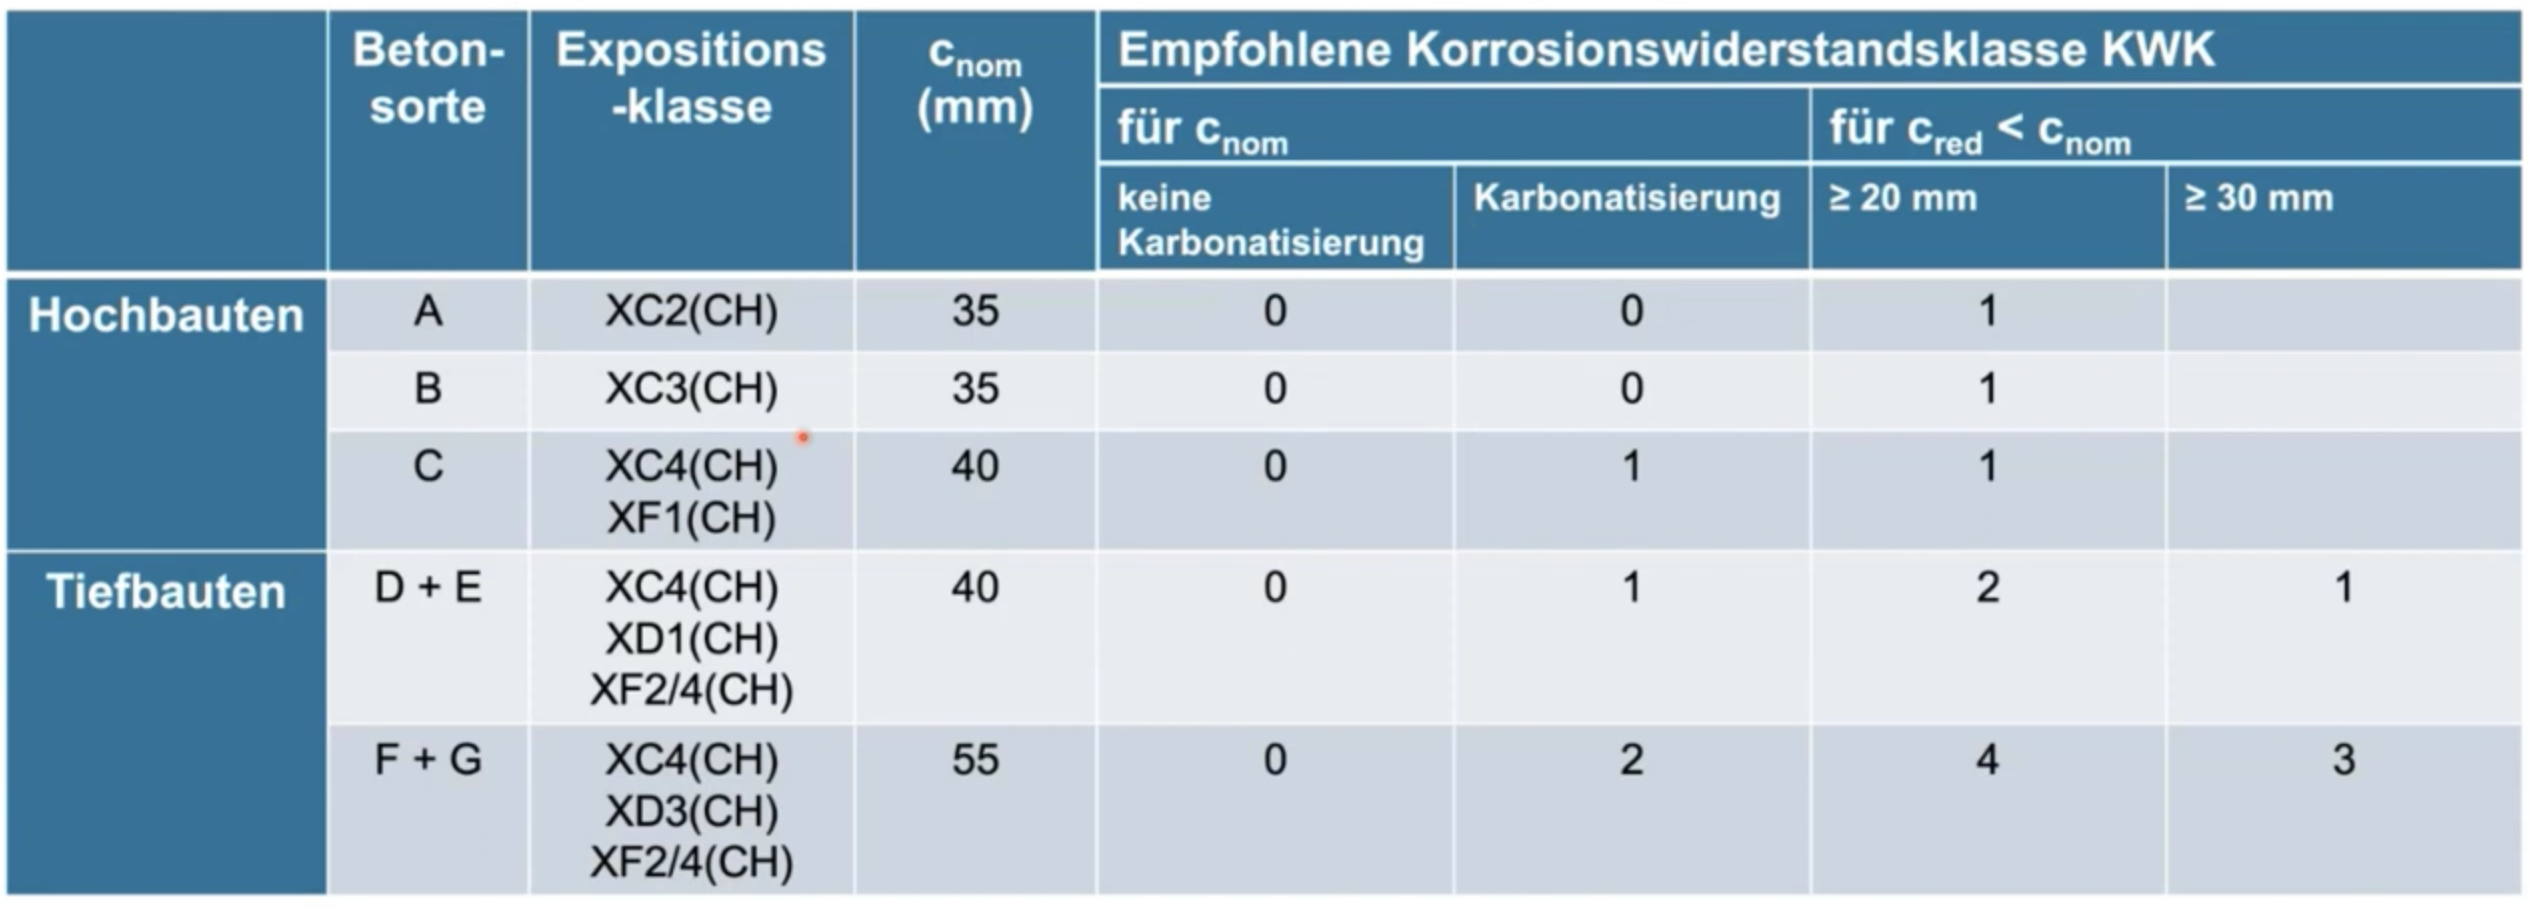
\includegraphics[width=1\linewidth]{/Users/patricpf/Documents/repos/Bauschule-Baustoffe/HTf-26/Bilder/Einteilung_Wirksumme.png}
        \caption{Quelle: SIA Merkblatt 2029, Tabelle 3}
    \end{figure}
    
\end{frame}


\begin{frame}{Korrosionsbeständige Bewehrung}
	\begin{block}{Video}
		\begin{itemize}
			\item [\textbullet] Weiter ab 15 min 
		\end{itemize}
	\end{block}
\end{frame}






\begin{frame}{Uploads auf Teams}
	\begin{itemize}
		\item[\textbullet] keine
	\end{itemize}
	        
\end{frame}
    
    
    
    
    

% \begin{frame}{Fragen zur Prüfung?}
        
% \end{frame}
    
\naechstePruefung{13.01.2024 }{Holz-und Holzwerkstoffe, Natursteine}
\folieFragen


\end{document}